\subsection{Classes de Complexidade}

\begin{definition}
    Dada uma medida de complexidade $\Phi$
    e uma função recursiva total
    $f: \mathbb N \rightarrow \mathbb N$,
    a \emph{classe de complexidade $f$} com relação a $\Phi$
    é o conjunto
    \begin{equation*}
        \mathcal C_\Phi(f) = \{ L(M) \mid \Phi(M, x) \leq f(|x|)
            \text{ para quase todos os $x$}
        \}.
    \end{equation*}
\end{definition}
Permitiremos que a complexidade de $M$
possa ser maior que $f$ para um número finito de elementos
para simplificar as demonstrações.

Embora faça sentido definir $\mathcal C_\Phi(f)$
para funções $f$ arbitrárias,
a exigência de $f$ ser recursiva total
torna as classes de complexidade
sucetíveis a argumentos por diagonalização.

Por exemplo,
podemos mostrar que
nenhuma classe de complexidade contém todas as linguagens recursivas.
Precisamos de um lema.

\begin{lemma}
    Existe um mapeamento bijetivo computável
    entre $\mathbb N$ e $\mathbb N \times \mathbb N$.
\end{lemma}

\begin{proof}
    Percorra o caminho descrito pelas setas na figura~\ref{passeio_cantor}.

    \begin{figure}[h]
        \centering
        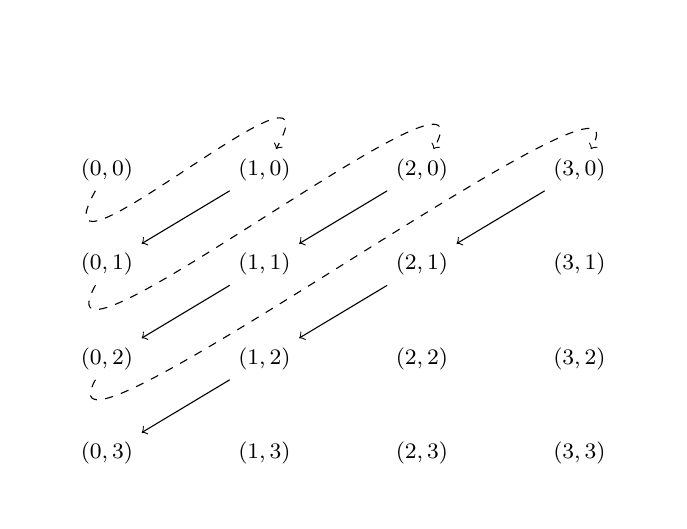
\begin{tikzpicture}
            \foreach \i in {0,...,3}
            \foreach \j in {0,...,3} {
                \node[font=\footnotesize]
                    (a\i\j) at (2*\i, -1.2*\j) {$(\i, \j)$};
            }

            \foreach \a/\b in {a00/a10, a01/a20, a02/a30} {
                \draw[->, dashed] (\a) .. controls
                +(-1,-1.8) and
                +(1, 1.8) .. (\b);
            }

            \foreach \a/\b in {
                a10/a01, a20/a11, a11/a02,
                a30/a21, a21/a12, a12/a03%
            } {
                \draw[->] (\a) -- (\b);
            }
        \end{tikzpicture}
        \caption{Passeio de Cantor.}
        \label{passeio_cantor}
    \end{figure}

    Em essência, primeiro enumeraremos todas os pares $(m, n)$
    para os quais $m + n = 0$,
    depois todos aqueles que $m + n = 1$,
    depois todos os que $m + n = 2$,
    e assim por diante.

    Esta técnica é conhecida como ``passeio de Cantor''
    \cite[p.~6]{CarnielliConiglioBianconi2006}.
\end{proof}

\begin{lemma}
    Existe uma função sobrejetora computavel
    $f: \mathbb N \rightarrow \mathbb N$
    tal que,
    para todo $y$,
    existem infinitos $x$ tais que $f(x) = y$.
\end{lemma}
\begin{proof}
    Considere $g$ como a função do lema anterior,
    e defina
    \begin{equation*}
        f(x) = y \quad \text{se} \quad g(x) = (y, z). \qedhere
    \end{equation*}
\end{proof}

\begin{lemma}
    Existe uma máquina de Turing $N$
    tal que $N(x)$ sempre está definido,
    e representa uma máquina de Turing,
    de forma que toda \emph{representação}
    de uma máquina de Turing
    é $N(x)$ para infinitamente muitos $x$.
    Isto é, $N$ produz todas as representações de máquinas de Turing
    infinitas vezes,
    conforme permitimos que $x$ tome valores arbitrários de $\Sigma^*$.
\end{lemma}

\begin{proof}
    Observe que existe uma bijeção computável
    entre palavras de $\Sigma^*$
    e números naturais.
    $N$ computará,
    dado um $x$,
    o número natural equivalente a ele
    e usar a função do lema anterior
    para gerar outro número.
    Então, $N$ converterá este outro número
    novamente para uma palavra de $\Sigma^*$.

    Todas as palavras de $\Sigma^*$
    são representações de máquinas de Turing;
    portanto, esta palavra produzida é a máquina desejada.

    Como a função do lema anterior
    produz todos números naturais infinitas vezes
    (e $N$ é capaz de suprir todos os números naturais
    como entrada para aquela função),
    todas as representações de máquinas de Turing
    são produzidas por $N$ infinitas vezes.
\end{proof}

\begin{theorem}
    Seja $\mathcal C_\Phi(f)$ uma classe de complexidade
    com relação à $\Phi$.
    Então existe uma linguagem $L$
    que não pertence à esta classe de complexidade.
    \label{funcao_fora_classe}
\end{theorem}

\begin{proof}
    Construiremos uma linguagem $L$
    que discorda de todas as máquinas de Turing que gastam menos de
    $f(n)$ recursos ao computar uma palavra de tamanho $n$.

    Usaremos a máquina $N$ do lema anterior.
    Denotaremos por $M_x$
    a máquina de Turing que $N$ produz
    ao lhe ser dada a palavra $x$.
    Colocarems $x$ em $L$
    de acordo com o comportamento que $M_x$ tem ao computar $x$.
    Caso esta máquina encerre sua computação
    gastando no máximo $f(|x|)$ recursos,
    executaremos"-na até o final da computação
    e inverteremos o resultado:
    se $M_x$ aceita $x$, então $x \notin L$;
    se $M_x$ rejeita $x$, então $x \in L$.
    Caso $M_x$ exiga mais do que $f(|x|)$ recursos,
    coloque $x$ em $L$.
    \footnote{
        Este argumento é,
        de certa forma,
        uma versão limitada
        (por $f$)
        do problema da parada.
    }

    Em outras palavras,
    \begin{equation*}
        L = \{ x \mid \text{
            $M_x$ não aceita $x$ gastando menos de $f(|x|)+1$ recursos
        } \}
    \end{equation*}

    Determinar se $M_x$ computa $x$ usando no máximo $f(|x|)$ de recursos
    é equivalente a determinar se $\Phi(M_x, x) = k$
    para algum $k \leq f(|x|)$.
    Como $f(|x|)$ é computável
    e ``$\Phi(M_x, x) = k$'' é decidível
    (pelo axioma~\ref{blum_rec}),
    esta verificação é realizável por uma máquina de Turing.
    Caso a resposta seja negativa
    ($M_x$ gasta mais do que $f(|x|)$ recursos ao computar $x$),
    já sabemos que $x$ está em $L$.
    Caso contrário,
    $\Phi(M_x, x)$ está definido;
    pelo axioma~\ref{blum_def},
    $M_x(x)$ também está.
    Portanto, podemos executar $M_x$ em $x$
    e inverter a resposta.

    Podemos computar $M_x$ e executar a operação descrita no parágrafo anterior;
    isso garante que $L$ é recursiva.

    Suponha agora que alguma máquina $M$ reconheça $L$.
    $M$ é $M_x$ para infinitos $x$ diferentes.
    $M$ aceita todos esses $x$
    e precisa fazê"-lo gastando mais do que $f(|x|)$ recursos,
    caso contrário $L$ discordaria de $L(M)$ nesses pontos.
    Portanto, $\Phi(M, x) \geq f(|x|)$ para infinitos $x$.

    Ou seja, qualquer máquina que aceite $L$
    precisa gastar mais de $f(|x|)$ recursos para infinitos $x$,
    portanto o predicado ``$\Phi(M, x) \leq f(|x|)$ para quase todos os $x$''
    não pode ser verdadeiro.
    Portanto,
    \begin{equation*}
        L \notin \mathcal C_\Phi(f). \qedhere
    \end{equation*}
\end{proof}
